\documentclass[12pt]{article}

\usepackage{answers}
\usepackage{setspace}
\usepackage{graphicx}
\usepackage{enumitem}
\usepackage{multicol}
\usepackage{circuitikz}
\usepackage{adjustbox}
\usepackage{mathrsfs}
\usepackage{svg}
\usepackage[margin=1in]{geometry} 
\usepackage{amsmath,amsthm,amssymb}
\setlength{\voffset}{-0.75in}
\setlength{\hoffset}{0in}
\setlength{\headsep}{0in}
\newcommand{\N}{\mathbb{N}}
\newcommand{\Z}{\mathbb{Z}}
\newcommand{\C}{\mathbb{C}}
\newcommand{\R}{\mathbb{R}}

\DeclareMathOperator{\sech}{sech}
\DeclareMathOperator{\csch}{csch}
 
\newenvironment{theorem}[2][Theorem]{\begin{trivlist}
\item[\hskip \labelsep {\bfseries #1}\hskip \labelsep {\bfseries #2.}]}{\end{trivlist}}
\newenvironment{definition}[2][Definition]{\begin{trivlist}
\item[\hskip \labelsep {\bfseries #1}\hskip \labelsep {\bfseries #2.}]}{\end{trivlist}}
\newenvironment{proposition}[2][Proposition]{\begin{trivlist}
\item[\hskip \labelsep {\bfseries #1}\hskip \labelsep {\bfseries #2.}]}{\end{trivlist}}
\newenvironment{lemma}[2][Lemma]{\begin{trivlist}
\item[\hskip \labelsep {\bfseries #1}\hskip \labelsep {\bfseries #2.}]}{\end{trivlist}}
\newenvironment{exercise}[2][Exercise]{\begin{trivlist}
\item[\hskip \labelsep {\bfseries #1}\hskip \labelsep {\bfseries #2.}]}{\end{trivlist}}
\newenvironment{solution}[2][Solution]{\begin{trivlist}
\item[\hskip \labelsep {\bfseries #1}]}{\end{trivlist}}
\newenvironment{problem}[2][Problem]{\begin{trivlist}
\item[\hskip \labelsep {\bfseries #1}\hskip \labelsep {\bfseries #2.}]}{\end{trivlist}}
\newenvironment{question}[2][Question]{\begin{trivlist}
\item[\hskip \labelsep {\bfseries #1}\hskip \labelsep {\bfseries #2.}]}{\end{trivlist}}
\newenvironment{corollary}[2][Corollary]{\begin{trivlist}
\item[\hskip \labelsep {\bfseries #1}\hskip \labelsep {\bfseries #2.}]}{\end{trivlist}}
\pagenumbering{gobble}
\begin{document}
 
% --------------------------------------------------------------
%                         Start here
% --------------------------------------------------------------
 
\title{Op - Amp}%replace with the appropriate homework number
\author{Aditya Arora\\ %replace with your name
Winter 2018} %if necessary, replace with your course title
 
\maketitle
%Below is an example of the problem environment

\begin{figure}[htbp]
  \centering
  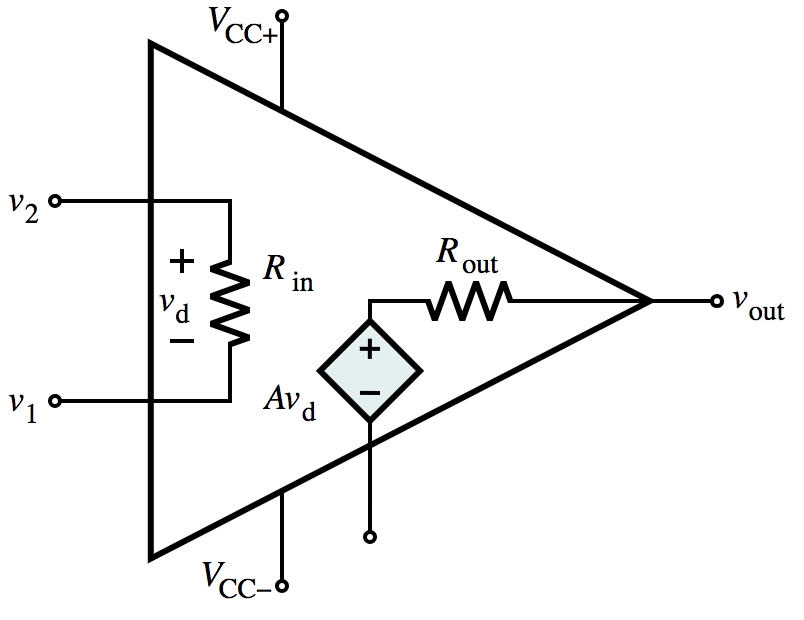
\includegraphics[scale=0.5]{internalopamp}
  \caption{Op-Amp Internal Structure}
\end{figure}
\begin{center}
${v_{d}  = v_{2}-v_{1}}$\\
${v_{o} = Av_{d}  = A(v_{2}-v_{1})}$
\end{center}


\section*{Ideal Op-Amp}
\textbf{TREAT AN OP-AMP AS A REGULAR CIRCUIT ELEMENT WITH JUST SPECIFIC CIRCUIT ELEMENT PROPERTIES
   \begin{trivlist}
    \item 1. No current ever flows into either input terminal.
    \item 2. There is no voltage difference between the two input terminals.
    \end{trivlist}
}

In a real op amp, a very small leakage current will flow into the input (sometimes as low as 40 femtoamperes). It is also possible to obtain a very small voltage across the two input terminals. However, compared to other voltages and currents in most circuits, such values are so small that including them in the analysis does not typically affect our calculations.


\pagebreak
\setlength{\voffset}{0.15in}
% \vskip 0.5in
% \begin{circuitikz}
%   \draw (0,0) node[op amp] (opamp) {}
%   (opamp.-) to [R, l_=$R_1$, *-o] ($(opamp.-)-(2,0)$) node[left]{$V_{in}$}
%   (opamp.-) |- ($(opamp.-)+(0.2,1)$) to[R=$R_2$] ($(opamp.-)+(2.2,1)$) -|
%   (opamp.out) to[short,*-] ($(opamp.out)+(.5,0)$) node [right] {$V_{out}$} node [ocirc] {} 
%   (opamp.+) to[short]  ($(opamp.+)-(0,.5)$) node[ground] {}
%   ;
% \end{circuitikz}


\begin{figure}[htbp]
  \centering
  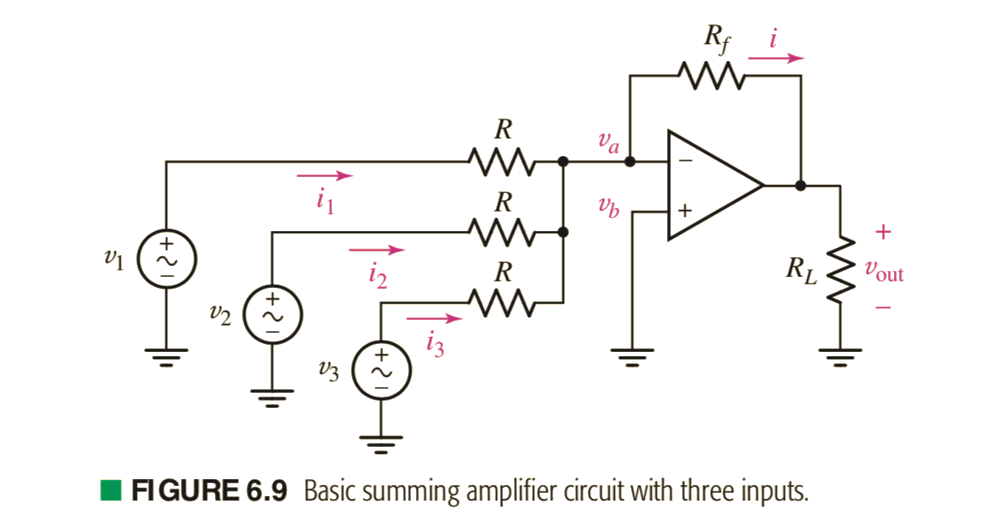
\includegraphics[scale=0.4]{warning}
\end{figure}
It is frequently tempting to assume that the current labeled i in Fig. 6.9 flows not only through $R_f$ but through $R_L$ also. Not true! It is very possible that current is flowing through the output terminal of the op amp as well, so that the currents through the two resistors are not the same. It is for this reason that we almost universally avoid writing KCL equations at the output pin of an op amp, which leads to the preference of nodal over mesh analysis when working with most op amp circuits.

\begin{figure}[htbp]
  \centering
  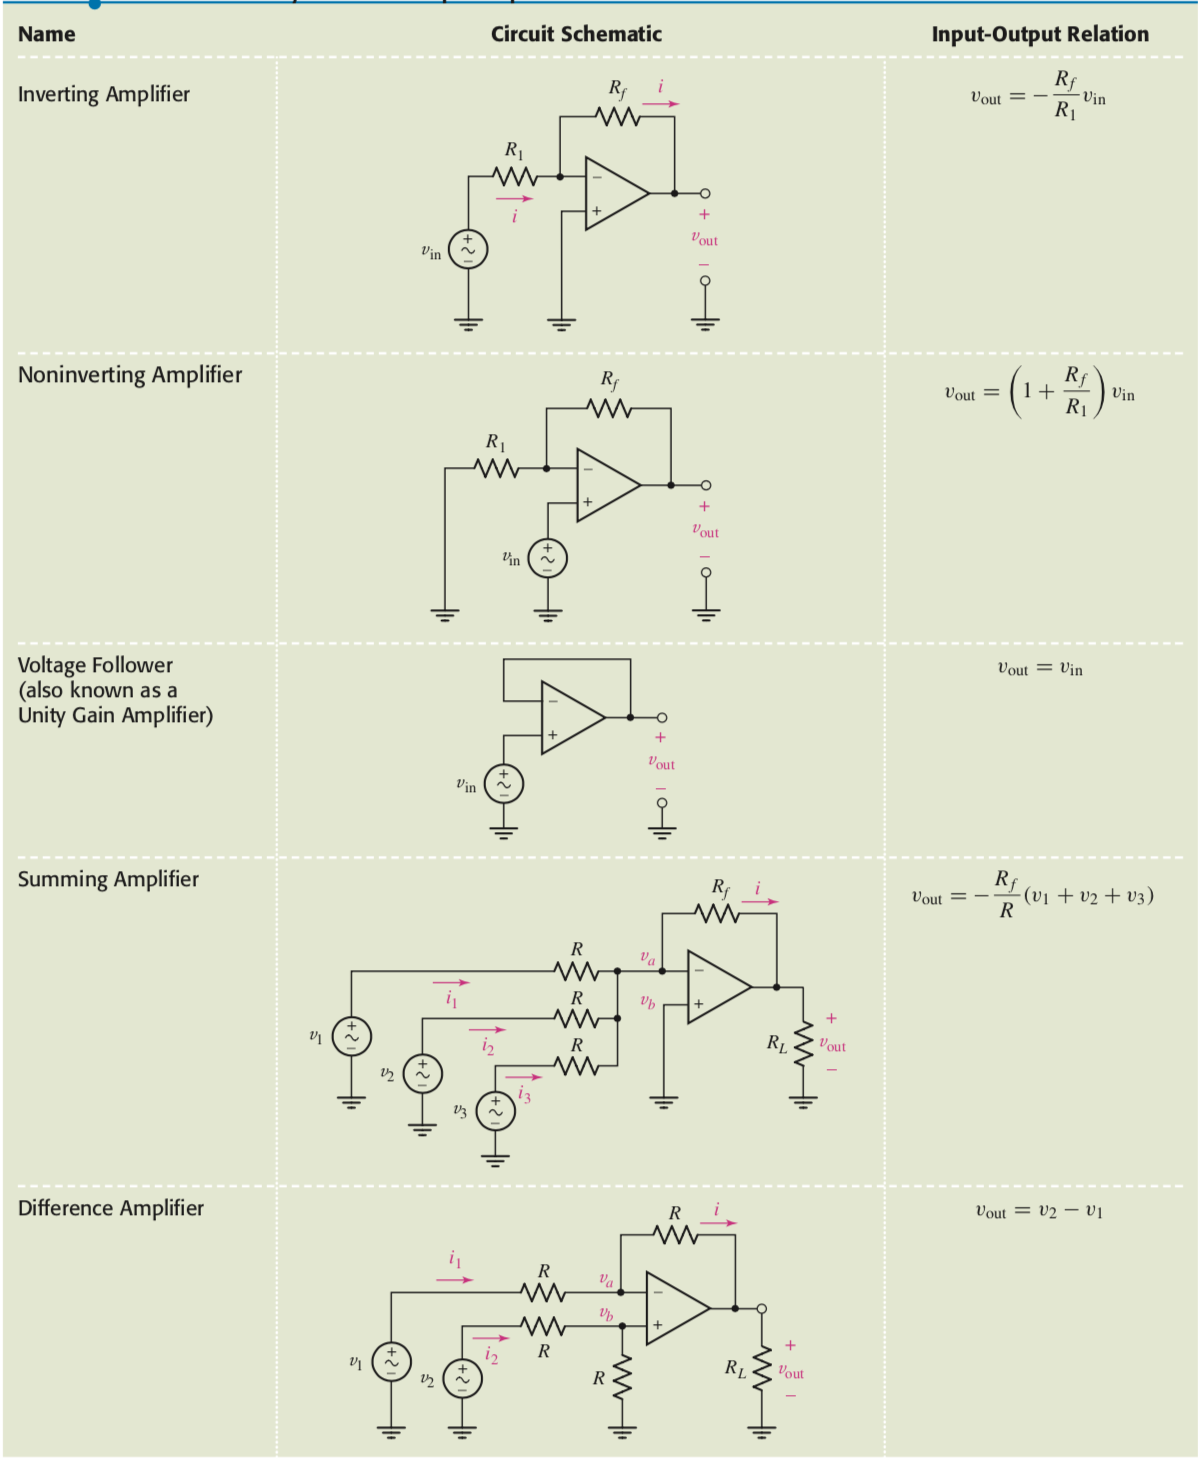
\includegraphics[scale=0.75]{OPAMP}
  \caption{Op-Amp Cheat Sheet}
\end{figure}
\end{document}
